% UML state machines for a batch job and for a prediction (Section 3.2).
\documentclass[tikz,border=1pt]{standalone}
% =====================================================================
%  Shared style for every diagram in the proposal.
%  Each figure is a standalone TikZ file that \input's this preamble, so
%  all diagrams use the same font family (Computer Modern, T1 -- identical
%  to the LLNCS body text), the same sizes and the same palette.
%
%  Font rule (do not change per figure):
%    node text   \footnotesize  (8 pt)
%    edge labels \scriptsize    (7 pt)
%    titles      \footnotesize\bfseries
%  Figures are drawn at their final width (<= 12.2 cm, the LLNCS text
%  width) and included WITHOUT scaling, so the printed size is the same
%  in every figure.
% =====================================================================
\usepackage[T1]{fontenc}
\usepackage{amsmath,amssymb}
\usepackage{xcolor}
\usepackage{tikz}
\usetikzlibrary{positioning,arrows.meta,shapes.geometric,shapes.multipart,
  fit,backgrounds,calc,shadows,patterns}

% ---- palette ---------------------------------------------------------
\definecolor{cBlue}{HTML}{0B4F8A}    % application / API
\definecolor{cOrange}{HTML}{B4540A}  % processing / services
\definecolor{cPurple}{HTML}{5B3CC4}  % data stores
\definecolor{cGreen}{HTML}{1B7A3A}   % success / output
\definecolor{cRed}{HTML}{B42318}     % error / risk
\definecolor{cGray}{HTML}{5F6672}    % external / neutral
\definecolor{cInk}{HTML}{1F2933}     % text and arrows

\colorlet{fBlue}{cBlue!9}
\colorlet{fOrange}{cOrange!10}
\colorlet{fPurple}{cPurple!9}
\colorlet{fGreen}{cGreen!10}
\colorlet{fRed}{cRed!9}
\colorlet{fGray}{cGray!8}

% ---- fonts -----------------------------------------------------------
\newcommand{\figfont}{\footnotesize}
\newcommand{\lblfont}{\scriptsize}
\newcommand{\code}[1]{\texttt{#1}}

\tikzset{
  every picture/.style={font=\figfont, line join=round, >={Stealth[length=4pt,width=3.4pt]}},
  every node/.append style={execute at begin node={\hyphenpenalty=10000\exhyphenpenalty=10000}},
  base/.style={draw, rounded corners=2pt, line width=0.6pt, align=center,
               inner xsep=3pt, inner ysep=2.5pt, text=cInk, font=\figfont},
  app/.style={base, draw=cBlue, fill=fBlue},
  svc/.style={base, draw=cOrange, fill=fOrange},
  data/.style={base, draw=cPurple, fill=fPurple},
  ok/.style={base, draw=cGreen, fill=fGreen},
  bad/.style={base, draw=cRed, fill=fRed},
  ext/.style={base, draw=cGray, fill=fGray},
  plain/.style={base, draw=none, fill=none},
  db/.style={cylinder, shape border rotate=90, aspect=0.22, draw=cPurple,
             fill=fPurple, line width=0.6pt, align=center, text=cInk,
             minimum height=9mm, font=\figfont},
  decision/.style={diamond, aspect=2.2, draw=cOrange, fill=fOrange,
                   line width=0.6pt, align=center, inner sep=1pt, text=cInk, font=\figfont},
  actor/.style={draw=cInk, fill=fGray, line width=0.8pt, rounded corners=0pt,
                align=center, inner sep=3pt, font=\figfont\bfseries},
  layer/.style={draw=cGray!60, fill=cGray!4, rounded corners=3pt, line width=0.5pt},
  layertitle/.style={font=\lblfont\bfseries, text=cGray, anchor=north west, inner sep=2pt},
  arr/.style={->, draw=cInk, line width=0.6pt},
  darr/.style={->, draw=cGray, line width=0.6pt, dashed},
  biarr/.style={<->, draw=cInk, line width=0.6pt},
  lbl/.style={font=\lblfont, text=cInk, inner sep=1.5pt},
  lblbg/.style={font=\lblfont, text=cInk, inner sep=1.5pt, fill=white},
}

% ---- UML sequence-diagram helpers -----------------------------------
%  \lifeline{id}{x}{label}{bottom y}   head box + dashed life line
%  \msg{x1}{x2}{y}{label}              synchronous call (solid)
%  \ret{x1}{x2}{y}{label}              reply (dashed)
%  \selfmsg{x}{y}{label}               call to self, label on the right
%  \fragment{kind}{guard}{x1}{y1}{x2}{y2}  combined fragment (alt/loop/par)
\newcommand{\lifeline}[4]{%
  \node[app, text width=19mm, minimum height=8.5mm, font=\figfont\bfseries] (#1) at (#2,0) {#3};
  \draw[cGray, dashed, line width=0.5pt] (#1.south) -- (#2,#4);}
\newcommand{\msg}[4]{%
  \draw[arr] (#1,#3) -- node[lbl, above] {#4} (#2,#3);}
\newcommand{\ret}[4]{%
  \draw[darr] (#1,#3) -- node[lbl, above] {#4} (#2,#3);}
\newcommand{\selfmsg}[3]{%
  \draw[arr] (#1,#2+0.12) -- ++(0.3,0) -- ++(0,-0.24) -- ++(-0.3,0);
  \node[lbl, anchor=west, align=left] at (#1+0.35,#2) {#3};}
\newcommand{\fragment}[6]{%
  \draw[cGray, line width=0.5pt] (#3,#4) rectangle (#5,#6);
  \node[anchor=north west, draw=cGray, fill=white, font=\lblfont\bfseries,
        inner sep=1.5pt, line width=0.5pt] at (#3,#4) {#1};
  \if\relax\detokenize{#2}\relax\else
  \node[anchor=north west, font=\lblfont, text=cGray, inner sep=1.5pt] at (#3+0.75,#4) {[#2]};\fi}
\newcommand{\activation}[3]{% x, y top, y bottom
  \draw[draw=cBlue, fill=fBlue, line width=0.5pt] (#1-0.07,#2) rectangle (#1+0.07,#3);}

\tikzset{
  st/.style={app, rounded corners=6pt, minimum width=20mm, minimum height=7mm},
  stok/.style={st, draw=cGreen, fill=fGreen},
  stbad/.style={st, draw=cRed, fill=fRed},
  init/.style={circle, fill=cInk, minimum size=2.2mm, inner sep=0},
  final/.style={circle, draw=cInk, line width=0.6pt, minimum size=3.2mm, inner sep=0,
                path picture={\fill[cInk] (path picture bounding box.center) circle (0.9mm);}},
}
\begin{document}
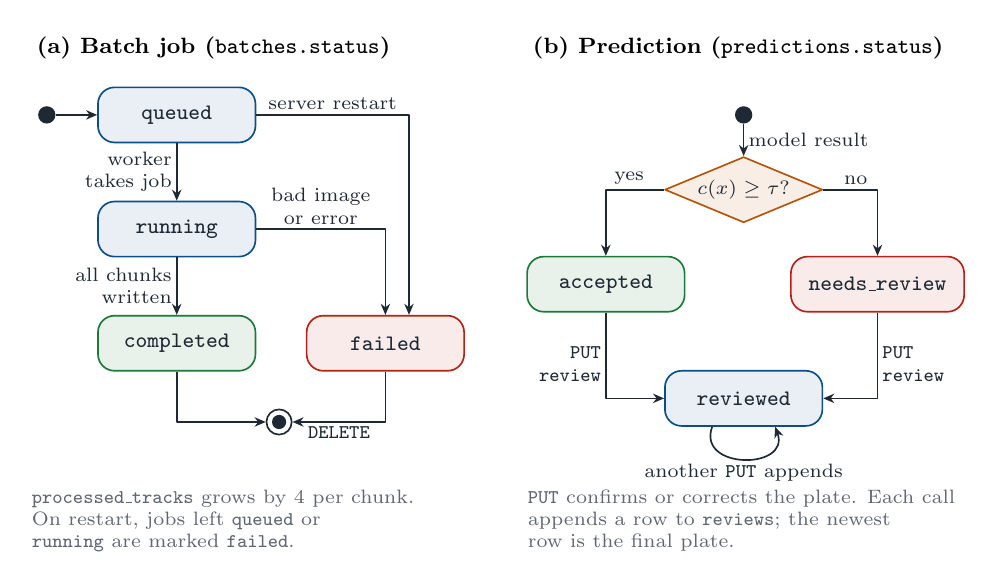
\begin{tikzpicture}
  % ---------------- (a) batch ----------------
  \node[font=\figfont\bfseries, anchor=west] at (0,0.55) {(a) Batch job (\code{batches.status})};
  \node[init] (b0) at (0.25,-0.3) {};
  \node[st] (q) at (1.9,-0.3) {\code{queued}};
  \node[st] (r) at (1.9,-1.75) {\code{running}};
  \node[stok] (c) at (1.9,-3.2) {\code{completed}};
  \node[stbad] (f) at (4.55,-3.2) {\code{failed}};
  \node[final] (bf) at (3.2,-4.2) {};
  \draw[arr] (b0) -- (q);
  \draw[arr] (q) -- node[lbl, left, align=right] {worker\\takes job} (r);
  \draw[arr] (r) -- node[lbl, left, align=right] {all chunks\\written} (c);
  \draw[arr] (r) -| node[lbl, pos=0.25, above, align=center] {bad image\\or error} (f);
  \draw[arr] (q) -| node[lbl, pos=0.25, above, align=center] {server restart} ([xshift=3mm]f.north);
  \draw[arr] (c.south) |- (bf);
  \draw[arr] (f.south) |- node[lbl, pos=0.75, below] {\code{DELETE}} (bf);
  \node[lbl, text=cGray, align=left, anchor=north west] at (0,-5.0)
    {\code{processed\_tracks} grows by 4 per chunk.\\On restart, jobs left \code{queued} or\\\code{running} are marked \code{failed}.};

  % ---------------- (b) prediction ----------------
  \begin{scope}[xshift=6.3cm]
  \node[font=\figfont\bfseries, anchor=west] at (0,0.55) {(b) Prediction (\code{predictions.status})};
  \node[init] (p0) at (2.8,-0.3) {};
  \node[decision, aspect=2.4, font=\lblfont] (g) at (2.8,-1.25) {$c(x)\ge\tau$?};
  \node[stok] (a) at (1.05,-2.45) {\code{accepted}};
  \node[stbad, minimum width=22mm] (n) at (4.5,-2.45) {\code{needs\_review}};
  \node[st] (v) at (2.8,-3.9) {\code{reviewed}};
  \draw[arr] (p0) -- node[lbl, right] {model result} (g);
  \draw[arr] (g) -| node[lbl, pos=0.3, above] {yes} (a);
  \draw[arr] (g) -| node[lbl, pos=0.3, above] {no} (n);
  \draw[arr] (a) |- node[lbl, pos=0.3, left, align=right] {\code{PUT}\\\code{review}} (v);
  \draw[arr] (n) |- node[lbl, pos=0.3, right, align=left] {\code{PUT}\\\code{review}} (v);
  \draw[arr] ([xshift=-4mm]v.south) .. controls +(-0.2,-0.55) and +(0.2,-0.55) .. node[lbl, below] {another \code{PUT} appends} ([xshift=4mm]v.south);
  \node[lbl, text=cGray, align=left, anchor=north west] at (0,-5.0)
    {\code{PUT} confirms or corrects the plate. Each call\\appends a row to \code{reviews}; the newest\\row is the final plate.};
  \end{scope}
\end{tikzpicture}
\end{document}
